\documentclass[aspectratio=169] {beamer}
%\documentclass[aspectratio=169, handout] {beamer}
%\usepackage{pgfpages}
%\usepackage{handoutWithNotes}
%\pgfpagesuselayout{2 on 1 with notes landscape}[a4paper,border shrink=1mm]  % No 16:9 mod for other settings 

%\useoutertheme{infolines}
\usetheme[left]{Goettingen}

\definecolor{NASAred}{RGB}{238, 41, 61}
\definecolor{NASAblu}{RGB}{26, 93, 173}
\definecolor{MONblu}{RGB}{23, 64, 138}

\usepackage[utf8]{inputenc}
\usepackage[T1]{fontenc}
\usepackage{fixltx2e}
\usepackage{graphicx}
\usepackage{longtable}
\usepackage{float}
\usepackage{wrapfig}
\usepackage{rotating}
\usepackage[normalem]{ulem}
\usepackage{amsmath}
\usepackage{textcomp}
\usepackage{marvosym}
\usepackage{wasysym}
\usepackage{amssymb}
\usepackage{amsthm}
\usepackage{amsfonts}
\usepackage{listings}
\usepackage{hyperref}
\usepackage[noabbrev]{cleveref}
\usepackage{algorithmic}
\usepackage[]{algorithm2e}
\usepackage{url}
\usepackage{booktabs}
\usepackage{syntax} % EBNF
\usepackage{pgfplots}
\usepackage[font=small,labelfont=bf,tableposition=top]{caption}
\DeclareCaptionLabelFormat{andtable}{#1~#2  \&  \tablename~\thetable}


\usepackage{pgfgantt}  % Gantt Diagramme in LaTeX 
\usepackage{pdfpages}

\usepackage{proof}  % Schlussformeln
\usepackage{bussproofs}  % Mehr Schlussformeln
%\usepackage{fontawesome}  % Great for writing AC\faBolt DC and marking errors in a proof! 

%  some notational arrangements:
\def\imp{\supset}  % consequence backwards.
\def\land{\mathbin\&}  % /\ -> &
\def\seq{\vdash}  % Sequenzen 

\newtheorem{hypotheses}{Hypotheses}  

\usepackage[style=authoryear,backend=biber]{biblatex}
\bibliography{bib.bib}


%  Libertine Font Family - Vorzueglich fuer Manuscripten
\usepackage{libertine}
%\usepackage{libertinust1math}
\usepackage{tgcursor}  % texttt Font fuer Libertinus

%\setbeamercolor{title}{bg=MONblu, fg=white} % title block on first slide
%\setbeamercolor{palette primary}{bg=MONblu, fg=white} %right-hand side of bottom
%\setbeamercolor{palette secondary}{bg=NASAred, fg=white} % center bottom
%\setbeamercolor{palette tertiary}{bg=MONblu,fg=white} % left bottom
%\setbeamercolor{palette quaternary}{bg=NASAred,fg=white} %
%\setbeamercolor{structure}{fg=MONblu} % box headings

%\setbeamercolor{section in toc}{fg=MONblu} % TOC sections
%\setbeamercolor{subsection in head/foot}{bg=NASAred,fg=white} %
%\setbeamercolor{item projected}{fg=MONblu, bg=white} %
%\setbeamercolor{frametitle}{fg=MONblu,bg=white} %
%\setbeamercolor{local structure}{fg=MONblu} %
%\setbeamercolor{item projected}{fg=MONblu,bg=white} %
%\setbeamertemplate{itemize item}{\color{MONblu}$\bullet$} %
%\setbeamertemplate{itemize subitem}{\color{MONblu}\scriptsize{$\bullet$}}%

\title[Short Title]{Long Title: Formal Aspects of Trusted Computing}
\author[H. Lauer]{Hagen Lauer\\ \scriptsize Supervisors: Prof. Dr. Gerhard Gentzen}
\institute[Monash]{Monash University}
\date{\today}

\setbeamertemplate{footline}[frame number]

\begin{document}

\begin{frame}
\titlepage
\centering
\includegraphics[width=.15\textwidth]{bilder/monash}
\end{frame}

\begin{frame}
  \frametitle{Outline}
  \tableofcontents
\end{frame}

\section{Introduction}

\begin{frame}
  \frametitle{Introduction - Virtualization and Cloud Computing}

  \begin{itemize}
    \item Developed in the 1960's - ``to allow for a computer to be used by two or more people, simultaneously''\footnote{\scriptsize DARPA request to MIT ~1963}
    \item Back then: major breakthrough as computing resources became available, no need to \emph{own} the computer.
    \item Today: Massively improved infrastructure, development, and deployment tools as well as a variety of new \emph{Cloud} paradigms.
  \end{itemize}
\end{frame}

\begin{frame}\frametitle{Introduction - \emph{X-as-a-Service} today}
	%\includegraphics[scale=.4]{lost}
	\begin{figure}
		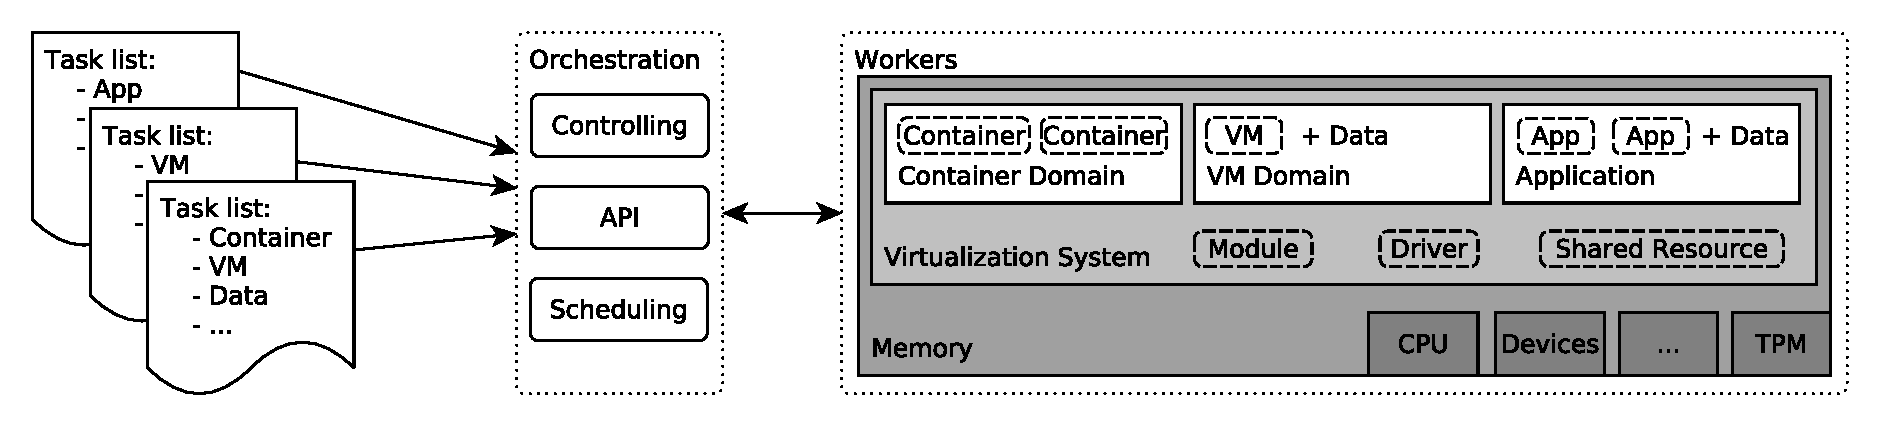
\includegraphics[scale=.4]{bilder/system-overview.pdf}
		\caption{An idealized abstraction of a virtualization system in the context of an orchestrated service architecture. The topology is sketched using shades of gray for lower layers. Boxes indicate domain separation and dashed lines distinguish threads and their memory from shared memory.}
	\end{figure}
\end{frame}

\begin{frame}\frametitle{Also today...}
\vfill
	\begin{minipage}{7cm}
		\includegraphics[scale=.4]{bilder/lost}
	\end{minipage}%
	\begin{minipage}{6cm}
		\begin{itemize}
			\item Quantifiable incentives for Cloud provider to cheat.
			\item Cloud computers can also be mis-configured or infected and provide an unsuitable environment.
		\end{itemize}
		In short, Cloud providers may be \emph{lazy}, \emph{dishonest}, or \emph{infected}.
	\end{minipage}
	\vfill
	{\scriptsize
	* \emph{2001: A Space Odyssey.}
	}
\end{frame}

\begin{frame}\frametitle{TCG-Model for Remote Verification}
	\begin{minipage}{6.5cm}
	Trusted Computing Group (TCG) offers:
		\begin{itemize}
			\item Founded early 2000's, lots of companies ... (and Monash!)
			\item \emph{Hardware protected} (encrypted) storage,
			\begin{itemize}
				\item Only \emph{authorized} software may encrypt data,
				\item e.g.: protecting FS root key, BitLocker ...
			\end{itemize}
			\item \emph{Attestation}: Prove to remote (server) what software started on machine.
		\end{itemize}
	\end{minipage}
	\hfill
	\begin{minipage}{5cm}
	Our motivation to pursue a TCG-model:
		\begin{itemize}
			\item \emph{Native applications} running on untrusted HW,
			\item \emph{Remotely verifiable} setup for services,
			\item \emph{Hardware roots of trust} for remote attestation.
		\end{itemize}
	\end{minipage}
\end{frame}

\begin{frame}\frametitle{TCG adds TPM to almost all PCs. What is it?}
\centering
\includegraphics[scale=.2]{bilder/boneh}\footnote{\scriptsize Credit: D.Boneh - Trusted Computing + SGX}
\begin{itemize}
	\item Trusted Platform Module (TPM), available on almost all relevant systems.
	\item Shares nothing with the rest of the system, has its own storage and processor.
	\item Supports all current \emph{standard} crypto primitives and gets updated constantly.
	\item \emph{Root-Keys} never leave the TPM.
\end{itemize}
\end{frame}

\begin{frame}\frametitle{PCRs, the most massively useful thing in the TPM}
	\textbf{PCR:} Platform Configuration Register
	\begin{itemize}
		\item Many PCR registers on a TPM (24+), since spec. v.2 even dynamically many.
		\item Content: SHA-$x$ wide SHA-$x$ digest
	\end{itemize}
	\vfill
	PCRs are special memory and can only be modified using \emph{extend}:
	\begin{itemize}
		\item TPM\_Extend(n,$v_{\nu}$): PCR(n) $\leftarrow$ $hash(\dots(hash(sinit||hash(v_1))\dots||hash(v_{\nu}))$ 
		\item consequently,
		\begin{itemize}
			\item we can not remove or overwrite entries,
			\item entries $sinit,\ v1,...,\ v_{\nu - 1}$ must have been extended \emph{before} $v_{\nu}$.
		\end{itemize}
	\end{itemize}
\end{frame}

\begin{frame}\frametitle{What is the point?}
\textbf{Attestation:} prove to remote party what software is loaded on my machine.
\begin{itemize}
	\item Good applications:
	\begin{itemize}
		\item Software can only run if machine runs patched OS.
		\item ...
	\end{itemize}
	\item Task owner can configure and specify the environment their workload should be running in ...
	%\item ... workloads can be monitored and tracked across compute nodes.
	%\item Works both ways: Cloud operators gain similar \emph{knowledge} and control over their infrastructure.
\end{itemize}
\vfill
\centering
\includegraphics[scale=.4]{bilder/attestation}
\end{frame}

\section{Sections}

\begin{frame}\frametitle{Overview}
	We will discuss the progress of our research using two research items:
	\vfill
	\begin{itemize}
		\item User-Centered Attestation for Layered and Decentralized Systems
		\begin{itemize}
			\item Remote attestation matters when defining standards
			\item Attestation must have explicit semantics and be trustworthy
		\end{itemize}
		\item The VS Metalanguage for Trusted Virtualization Systems
		\begin{itemize}
			\item Trusted platforms and trustworthy computers must have certain properties
			\item Current measurement architectures produce ambiguous evidence for attestations
			\item Evidence must be structured reflect target system topology
		\end{itemize}
	\end{itemize}
\end{frame}

\subsection{Subsection: User-Centered Attestation in Layered and Decentralized Systems}

\begin{frame}\frametitle{User-Centered Attestation in Layered and Decentralized Systems}
\textbf{Published at NDSS DISS 2018}.
\vfill
\uline{D}ecentralized \uline{I}oT \uline{S}ecurity and \uline{S}tandards\footnote{\scriptsize As stated by IETF}:
\begin{itemize}
	\item Decentralized approach to IoT security:
	\begin{itemize}
		\item Operating with constrained device and network capabilities
		\item State synchronization
		\item Trust management
	\end{itemize}
	\item Many IoT standards are now under development:
	\begin{itemize}
		\item Lots of different groups and standards bodies ...
		\item Systems composed of multiple standards also raise challenges
		\begin{itemize}
			\item e.g., how to maintain security across bridges and how to evaluate trust across standards boundaries.
		\end{itemize}
	\end{itemize}
\end{itemize}
\end{frame}

\begin{frame}\frametitle{Our Contribution}

\textbf{UCAS}: User-centered Attestation in Layered and Decentralized Systems.
\vfill

  \begin{itemize}
  \item We introduce technological and standardization efforts towards trustworthy Cloud computations
  \item outline challenges and potential conflicts related to translating \emph{trust} across standards
  \item evaluate current trust establishment methods and put them into a decentralized perspective
  \item propose User-centered Attestation as a candidate for layered and decentralized systems.
  \end{itemize}
\end{frame}

\begin{frame}[fragile]\frametitle{Zeugs}
  Dies und jenes ...
\end{frame}


\begin{frame}\frametitle{Hypotheses}
\begin{hypotheses}[Attestation must be User-Centered] (Informal)\\
\emph{Trust} placed originally only in hardware components needs to be extended to reporting and measurement mechanisms in upper layers.\\ 


Semantics of existing approaches are ambiguous...\\ 


Existing attestation approaches imply a particular topology, connectivity, and capability that does not reflect decentralized systems.\\ 


A \emph{User-Centered Attestation}, as a novel attestation system, must encompasses these concerns and proposes a strategy for specifying and synthesizing suitable trust establishment mechanisms. 
\end{hypotheses}
\end{frame}

\subsection{Subsection 2: The Virtualized Systems Metalanguage}

\begin{frame}\frametitle{Our Contribution: Formal Abstractions and Verification}
The \uline{V}irtualized \uline{S}ystems \uline{M}eta\uline{l}anguage, submitted to Euro S+P.
\vfill
\textbf{Formal Abstractions} of
\begin{itemize}
	\item \textbf{Trusted Systems:} \emph{Universal} Virtualization System (inspired by literature, Cloud use-cases, and standards)
	\item \textbf{TCG-based Computing Architectures:} Formal verification of measurement and recording strategy of evidence based on a static root of trust for measurement (SRTM) boot process\footcite{Gasser1989,Parno2010,Parno2011} and extensions into application space\footcite{Sailer2004}.
\end{itemize}
%Also introduces and formally verifies an Enhanced Integrity Measurement Architecture (EIMA) as an improvement to IMA in accordance with \emph{UCAS}.
\end{frame}

\begin{frame}\frametitle{Contribution of \emph{VSML} Paper}
Paper in progress.
\vfill
\begin{itemize}
	\item We introduce the VSML environment
	\item We demonstrate the capabilities of VSML by proving a well-known integrity measurement architecture
	\item The architecture does not meet the requirements and might even lead to insecure interactions
	\item We present and prove correct an enhancement and formally verify its trust property
\end{itemize}
\end{frame}

\begin{frame}\frametitle{Why formal abstractions? 20+ Million reasons...}
Statistics\footnote{\scriptsize https://www.linuxcounter.net/statistics/kernel} of the Linux Kernel alone:
\begin{itemize}
	\item It's a dirty place! 300+ swear words in the kernel code,
	\item \textbf{20+ Million} lines of code as of today...
\end{itemize}
\centering
\includegraphics[scale=0.2]{bilder/kernelstat}
\end{frame}

\begin{frame}\frametitle{Pictures: Shoulders we stand on.}
	\small
	\begin{minipage}{3cm}
		\centering
 		\includegraphics[scale=0.2]{bilder/gentzen}
 		\begin{itemize}
 			\item Gerhard Gentzen
 			\item Natural Deduction
 			\item Sequent Calculus
 			\item Proof theory
 		\end{itemize}
	\end{minipage}
	\hfill
	\begin{minipage}{3cm}
		\centering
 		\includegraphics[scale=0.05]{bilder/milner}
 		\begin{itemize}
 			\item Robin Milner
 			\item Standard ML
 			\item Language Semantics
 			\item Reduction based OS
 		\end{itemize}
	\end{minipage}
	\hfill
	\begin{minipage}{3cm}
		\centering
 		\includegraphics[scale=0.2]{bilder/carl}
 		\begin{itemize}
 			\item Carl Hewitt
 			\item Actor Model
 			\item ... everything is an Actor!
 		\end{itemize}
	\end{minipage}
	\hfill
	\begin{minipage}{3cm}
		\centering
 		\includegraphics[scale=0.22]{bilder/allen}
 		\begin{itemize}
 			\item James F. Allen
 			\item Interval Temporal Logic
 			\item Proof system
 		\end{itemize}
	\end{minipage}
\end{frame}

\begin{frame}\frametitle{The Virtualized Systems Metalanguage (\emph{VSML})}
	What is \emph{VSML}?
	\vfill
	\emph{VSML} is a three part formal system consisting of 
	\begin{itemize}
		\item a functional programming interface based on impure languages
		\item reduction based operational semantics
		\item first oder logic with hybrid modal extensions.
	\end{itemize}
\end{frame}

\begin{frame}\frametitle{More content}
...
\end{frame}


\begin{frame}\frametitle{Inline math}
The operational semantics are defined as a set of reduction rules \footcite{CCS,Milner1997,PICal} for each core construct which when applied to a state produces its successor.
\begin{itemize}
	\item Sequences of states $\mathcal{S}_{0} \xrightarrow{(f)} \mathcal{S}_{1} \xrightarrow{(f)} ... \xrightarrow{(f)} \mathcal{S}_{n}$ by applying reduction rules.
	\item Can be labeled with covariant counter $t$ $\mathcal{S}_{0} \xrightarrow{t} \mathcal{S}_{1} ... \xrightarrow{t_n} \mathcal{S}_{n}$. 
	\item ... this is how relative time $t$ is established.
\end{itemize}
\end{frame}

\begin{frame}\frametitle{Citations}
	\begin{itemize}
		\item Hybrid modal operator $@_t$ to signify that at some $t$ the Formula is true\footcite{Blackburn2000, Blackburn2006, Brauner2011}.
		\item $\Delta_{(t_{\mu},t_{\nu})}$ to express that for every $t, t_{\mu}<t<t_{\nu}$ the Formula is true~\footcite{Allen1983,Allen1984,Allen1989,Allen1994}.
	\end{itemize}
\end{frame}


\begin{frame}\frametitle{Theorems, Definitions}
\begin{definition}[SRTM Boot Sequence]\label{def:srtm}
\small
\begin{align*}
  & SRTM(m,t) = \exists t_{S},t_{B},t_{O},I\ .\ (t_{S}<t_{B}<t_{O}<t)\\
  & \qquad ...
\end{align*}
\begin{theorem}[Trustworthiness of SRTM Integrity Measurement]\label{thm:srtm} 
The following is provable in VSML:
\begin{align*}
  %&ProtectedCRTM(m)\ \land\\  &
  &Let\ seq\ = \ \langle sinit,BL(m),OS(m),APP(m)\rangle\\
  &TrustPlatform(m), @_t Mem(m.pcr.srtm,seq) \seq @_t SRTM(m,t)
\end{align*}
\end{theorem}
\end{definition}
\end{frame}

\section{Table}

\begin{frame}\frametitle{Tabellen}
\begin{table}[h]
\scriptsize
\centering
\caption{A caption.}
\begin{tabular}{lll}
Chapter & Title & Completion \\
\hline
1 & Introduction  & 80\% \\
2 & Problem Statement and Literature Review & 90\%  \\
3 & Formal Abstractions and Conceptual Framework& 50\% \\
3.1 & Functional Trust Model & 50\% \\
4 & Trust Establishment and Bootstrapping Trust &  60\%\\
4.1 & ... & ...\%\\
5 & Discussion & ...\\
5.1 & Formal Abstractions & ...\\ % Erweiterungen des TPMs, Agenten mit Wissen, verteilte Systeme
6 & Future Directions and Implications & ... \\
\end{tabular}
\end{table}
\end{frame}

\section*{Questions}

\begin{frame}
\centering
\Large
Thank you.
\end{frame}

\end{document}
